\documentclass{article}
\usepackage{package}
\graphicspath{ {./images/} }

\makeindex


\title{
    {\LARGE DONE - Docker Orchestrator for Network Emulation}\\
    \vskip 0.1cm{\Large Studio di fattibilità}
    %\vskip 0.8 cm{\Large Facolt\`a di Scienze e Tecnologie}\\
    \vskip 0.4cm{\large CdL in Sicurezza dei Sistemi e delle Reti Informatiche}
}
\author{
    \Large Samuele Manclossi, Melissa Moioli, Tiziano Radicchi\\
    \large 09882A, 09831A, 12172A
}
\date{
    {\large\today}
}

\makeatletter
\newcommand{\@alphalph}{}% Check that \@alphalph is undefined.
\let\@alphalph=\alphalph
\makeatother


\begin{document}
\pagenumbering{gobble}

\begin{titlepage}
    \pagestyle{empty}
    \selectlanguage{italian}
    \maketitle
    \selectlanguage{italian}
    \vspace{1em}
    \epigraph{\say{Non quia difficilia sunt non audemos, sed quia non audemos difficilia sunt}}{--- \textup{Seneca}}
    \selectlanguage{english}
    \vspace{2em}
    \begin{abstract}
        \textit{\noindent
Si propone lo studio di fattibilità per la proposta di progetto "DONE": la creazione di uno strumento, ispirato a IMUNES, per l'emulazione di reti mediante l'utilizzo automatizzato di Docker, interfaccia grafica e/o terminale.
\newline\newline
Esso si basa sugli stessi principi di virtualizzazione alla base di altri software di emulazione di reti. L'obiettivo è quello di fornire un ambiente di sviluppo e test per reti complesse, in modo da poter testare nuove configurazioni di rete e nuovi servizi senza dover ricorrere a costosi e complessi apparati fisici, garantendo allo stesso momento dipendenze da pochi strumenti quali Docker, OpenVSwitch e la segregazione dei namespaces offerta dai sistemi operativi Linux.
\newline\newline
Il nostro studio si concentrerà su tre macroargomenti: la virtualizzazione delle topologie di rete, la logica di emulazione e la logica di interazione, che permetterà all'utente di interagire con il programma sia tramite interfaccia grafica che da terminale.}
        %\textit{\kant[1]}% TODO 
    \end{abstract}
    \vskip 4cm\centerline{
\includegraphics[height=50mm]{./src/unimi}}
    \newpage
    \pagenumbering{Roman}
    \tableofcontents
    \selectlanguage{italian}
    \vspace{\fill}
\end{titlepage}

\pagenumbering{arabic}
\lhead{
    DONE - Studio di fattibilità
}
\rhead{Manclossi, Moioli, Radicchi}

\selectlanguage{italian}

\section{Introduzione}
Alla luce delle funzionalità che gli emulatori di rete oggi esistenti offrono, desideriamo, con l'obiettivo di approfondire le nostre conoscenze in ambito di reti e di sviluppo software, proporre una soluzione alternativa che offra feature extra ed un miglioramento generale della qualità di utilizzo.
\subsection{Funzionalità}
Le funzionalità che desideriamo offrire attraverso l'utilizzo di \texttt{DONE} sono le seguenti: 
\begin{itemize}
    \item L'utente può creare, aprire, modificare progetti di topologie di rete, aggiungendo apparati, definendo collegamenti tra questi, nonché fare uso di device specifici volti al collegamento della topologia definita a reti esterne alla simulazione. I dispositivi utilizzabili sono hub, switch, nodi, router, connessioni a interfacce esterne, con NAT o meno.
    \item Una volta realizzata la topologia desiderata, l'utente può salvare su file il progetto, con lo scopo di poter riprendere il lavoro in un secondo momento
    \item L'utente può assegnare per ogni singolo device delle configurazioni, che verranno applicate all'avvio della simulazione
    \item L'utente può avviare la simulazione, con la possibilità in seguito di accedere tramite terminale ai singoli nodi per aggiungere ulteriori configurazioni, per testare la connettività e/o effettuare troubleshooting. Il tutto esclusivamente tramite linea di comando. I nodi possono ospitare vari servizi, come ad esempio server ssh, ftp e web, anch'essi configurabili attraverso linea di comando. 
\end{itemize}
Gli obiettivi che desideriamo perseguire attraverso questo progetto sono:
\begin{itemize}
    \item \textbf{Ridurre le dipendenze} al minimo necessario, in modo da rendere il programma il più portabile possibile
    \item Fornire la \textbf{capacità di salvare} non solo la topologia fisica ma anche tutte le configurazioni, senza bisogno di script ulteriori
    \item \textbf{Maggiore pulizia dell'ambiente}, evitando che Docker rimanga in uno stato intermedio (ossia con i vecchi container ancora presenti) in caso di chiusura della applicazione senza arresto della simulazione, nonché pulizia dalle altre interfacce e apparati virtuali creati
    \item Offrire una soluzione open-source che possa essere \textbf{estesa} e \textbf{modificata}
\end{itemize}
\subsection{Architettura}
Alla luce delle funzionalità desiderate, l'architettura che abbiamo ideato per raggiungere gli obiettivi preposti è così organizzata: 
\begin{center}
    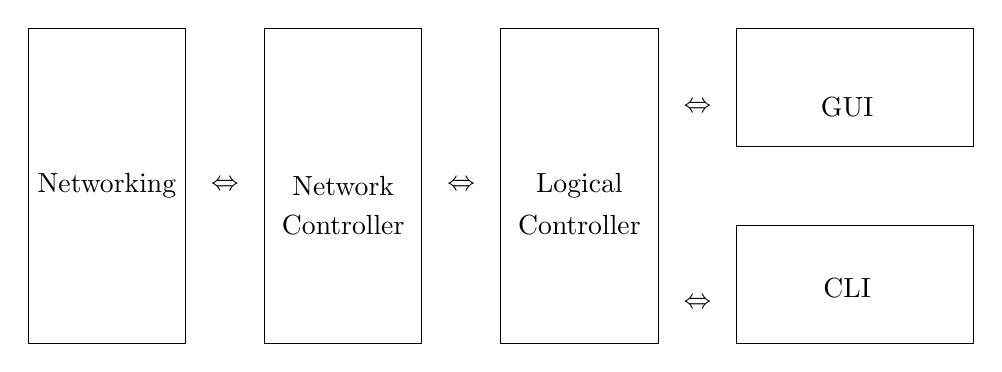
\begin{tikzpicture}
        \draw (12,0) rectangle (15, 1.5);
        \draw (12,2.5) rectangle (15,4);
        \draw (11,0) rectangle (9,4);
        \draw (8,0) rectangle (6,4);
        \draw (3,0) rectangle (5,4);
        \node[] at (4,2) {Networking}; 
        \node[] at (7,2) {Network};
        \node[] at (7,1.5) {Controller};
        \node[] at (10,2) {Logical};
        \node[] at (10,1.5) {Controller};
        \node[] at (13.4,0.7) {CLI};
        \node[] at (13.4,3) {GUI};
        \node[] at (5.5,2) {$\Leftrightarrow$};
        \node[] at (8.5,2) {$\Leftrightarrow$};
        \node[] at (11.5,0.5) {$\Leftrightarrow$};
        \node[] at (11.5,3) {$\Leftrightarrow$};
    \end{tikzpicture}
\end{center}
%\begin{center}
%    \begin{tikzpicture}
%        \node[rectangle,draw,minimum height=4cm,minimum width=2.5cm] at (5,4) {Networking};
%        \node[rectangle,draw,minimum height=4cm,minimum width=2.5cm] at (2,4) {Network Controller};
%    \end{tikzpicture}
%\end{center}

Pertanto, le componenti da realizzare sono:
\begin{itemize}
    \item \textbf{Networking}: Utilizzo di container e apparati virtualizzati. Si tratta del modo in cui vengono realizzati, come in IMUNES, i componenti veri e propri. Essi sono poi connessi tra di loro mediante gli appositi comandi e possono simulare una rete. Sarà gestito dal relativo controller attraverso utilizzo di librerie apposite sviluppate ad hoc.
    \item \textbf{Network Controller}: Automatizzazione, a fronte di una topologia creata, della creazione della configurazione di rete
    \item \textbf{Logical Controller}: Logica di controllo, a più alto livello, che possa gestire:
          \begin{itemize}
              \item Strutture per gestire la topologia creata
              \item Salvataggio della topologia
              \item Gestione e salvataggio delle configurazioni
              \item Invio delle informazioni necessarie al network controller per realizzare la topologia creata
          \end{itemize}
    \item \textbf{GUI}: si tratta dell'interfaccia su cui l'utente può disegnare la topologia logica della rete, posizionando quindi nodi e link tra nodi, trascinandoli, modificandoli e interagendoci in genere
    \item \textbf{CLI}: da qui si possono lanciare i comandi di configurazione dei vari componenti. Essa aprirà un editor di testo sui file di configurazione, permettendo quindi di modificarli, salvarli e caricare le modifiche anche nella visualizzazione GUI. Permetterà di accedere a CLI dedicate ai singoli nodi per inserire configurazioni
\end{itemize}


\newpage




\newpage
\end{document}
